\documentclass[10 pt,usenames,dvipsnames, oneside]{article}
\usepackage{../../../modelo-ensino-medio}



\begin{document}

\begin{center}
  \begin{minipage}[l]{3cm}

\includegraphics[width=2cm]{logo}    
\end{minipage}\hfill
\begin{minipage}[r]{.8\textwidth}
 {\Large \scshape Atividade: Potência de uma Lâmpada}  
\end{minipage}
\end{center}
\vspace{.2cm}

\ifdefined\prof
%Habilidades da BNCC
% \begin{objetivos}
% \item 
% \end{objetivos}

%Caixa do Para o Professor
\begin{goals}
%Objetivos específicos
\begin{enumerate}
\item Representar graficamente um intervalo.
\item Compreender um intervalo como solução de desigualdades simultâneas.
\end{enumerate}

\tcblower

%Orientações e sugestões
Tranquilize seus alunos com relação aos valores dessa atividade. Eles podem achar que estão seguindo pelo caminho errado porque os valores encontrados não são números inteiros, no entanto, lembre-os que os valores encontrados na realidade são assim mesmo.
\end{goals}

\bigskip
\begin{center}
{\large \scshape Atividade}
\end{center}
\fi

As redes elétricas de alguns estados do Brasil são projetadas para receberem uma tensão de 127V (Volts), porém existe uma variação natural nesse valor. As concessionárias estipulam uma variação máxima entre 116V e 133V e todos equipamentos fabricados no país são testados para suportar essa variação de tensão. Oscilações maiores na rede elétrica podem comprometer a potência dos eletrodomésticos e até mesmo avariá-los.

A potência de uma lâmpada está relacionada à tensão da rede elétrica e à resistência da lâmpada. Em Física, verifica-se que essa relação se dá através da seguinte fórmula:
$$
V = \sqrt{P\cdot R},
$$
onde $P$ representa a potência da lâmpada, medida em \emph{Watts} (W), $V$ é a tensão da rede medida em \emph{Volts} (V) e $R$ é a resistência da lâmpada medida em \emph{Ohms} ($\Omega$). Suponha que uma lâmpada de quintal tenha uma resistência de 144$\Omega$. O gráfico de $V$ em função $P$ é dado na figura abaixo: 

\begin{figure}[H]
\centering
\noindent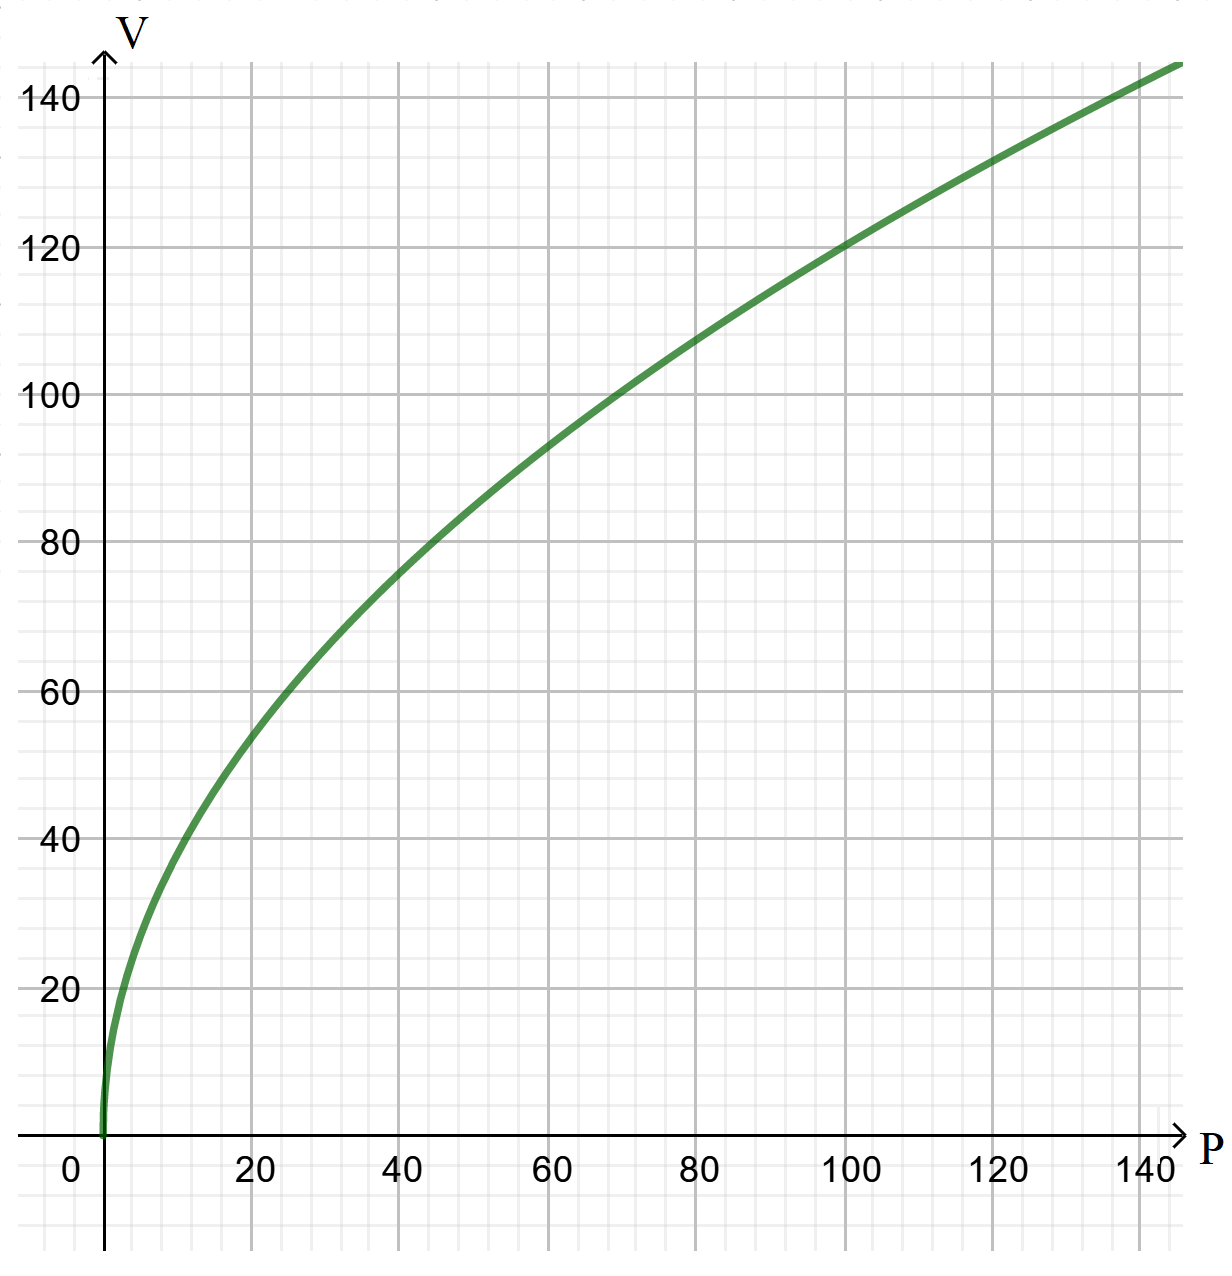
\includegraphics[width=200bp]{lampada}
\end{figure}

\begin{enumerate}
\item{}
Desenhe no eixo vertical o segmento que corresponde ao intervalo de variação de valores da tensão da rede estipuladas pelas concessionárias brasileiras.

\item{}
Desenhe no eixo horizontal, o segmento que corresponde ao intervalo de variação da potência da lâmpada, sabendo-se que a tensão $V$ oscila no intervalo $116\leq V \leq 133$. Em seguida, calcule o valor mínimo e máximo atingidos pela potência desta lâmpada.
\end{enumerate} 


\ifdefined\prof
\begin{solucao}

\begin{enumerate}
\item No eixo $Oy$ marque o intervalo $[116,133]$.
\item  Os valores aproximados de $P$ que correspondem às voltagens de $116V$ e $133V$ respectivamente são $93{,}4$ W e $122{,}8$W, assim, marque no eixo $Ox$  o intervalo $[93{,}4;122{,}8]$.
\end{enumerate}

\end{solucao}
\fi

\end{document}